%***********************************************************************************************************************************************************************************************
\subsection[GP PC Metamodel Construction]{\gls[hyper=false]{gp} \gls[hyper=false]{pc} Metamodel Construction: Training, Validation, and Selection}\label{sub:gp_feba_pca_metamodel_construction}
%***********************************************************************************************************************************************************************************************

% Introductory paragraph
Following the \gls[hyper=false]{pca} of the multivariate output, 
\gls[hyper=false]{gp} metamodels were constructed with respect to the standardized \gls[hyper=false]{pc} scores for each of the output types.
The effect of several factors potentially affecting the predictive performance of the \gls[hyper=false]{gp} metamodels were also investigated,
including training sample size as well as the choice of experimental design and covariance kernel function.

% PC GP Metamodel, Clad Temperature Output
It was found that higher \glspl[hyper=false]{pc} tends to be harder to fit.
\marginpar{\gls[hyper=false]{gp} \gls[hyper=false]{pc} metamodel, clad temperature output}
That is, more and more training samples were required to have a \gls[hyper=false]{gp} metamodel of good predictive accuracy.
Fig.~\ref{fig:ch4_plot_pc_q2_tc} shows the predictivity coefficient $Q_2$ as function of the training sample size for three different \glspl[hyper=false]{pc} \gls[hyper=false]{gp} metamodels with respect to the clad temperature output.
The $Q_2$ was calculated based on the validation data set of $5'000$ data points (i.e., independent \gls[hyper=false]{trace} runs).
The multiple points per training sample size correspond to \gls[hyper=false]{gp} metamodels constructed using different experimental designs, covariance kernel functions, and the five replications.
\bigfigure[pos=!tbhp,
					 opt={width=0.82\textwidth},
           label={fig:ch4_plot_pc_q2_tc},
           shortcaption={Convergence of \gls[hyper=false]{pc} metamodel with increasing number of training samples with respect to the standardized \glspl[hyper=false]{pc} scores associated with the clad temperature output}]
{../figures/chapter4/figures/plotPCQ2TC}
{Convergence of \gls[hyper=false]{pc} metamodel with increasing number of training samples with respect to the \glspl[hyper=false]{pc} scores associated with the clad temperature output and the $Q_2$ validation metric. The number inside parentheses is the explained variance of the output by the \gls[hyper=false]{pc} and the cumulative explained variance of the first $10$ \glspl[hyper=false]{pc} is about $96\%$.}

The leftmost panel of the plot shows that indeed the \gls[hyper=false]{gp} metamodel for the first standardized \gls[hyper=false]{pc} score is the easiest to fit,
requiring only a small size of training sample.
On the other hand, the rightmost panel of the plot shows that not even the largest number of training samples considered is enough to have a \gls[hyper=false]{gp} metamodel with decent performance for the $10$\textsuperscript{th} \gls[hyper=false]{pc}.
Furthermore, the plot also shows that the variations in the performance tends to become smaller with increasing sample size.

% (negative and zero predictivity coefficient means that no benefit is gained from using \gls[hyper=false]{gp} metamodel to make the prediction)

% PC GP Metamodel Construction, Clad Temperature Output
\begin{sidewaysfigure}
	\centering
	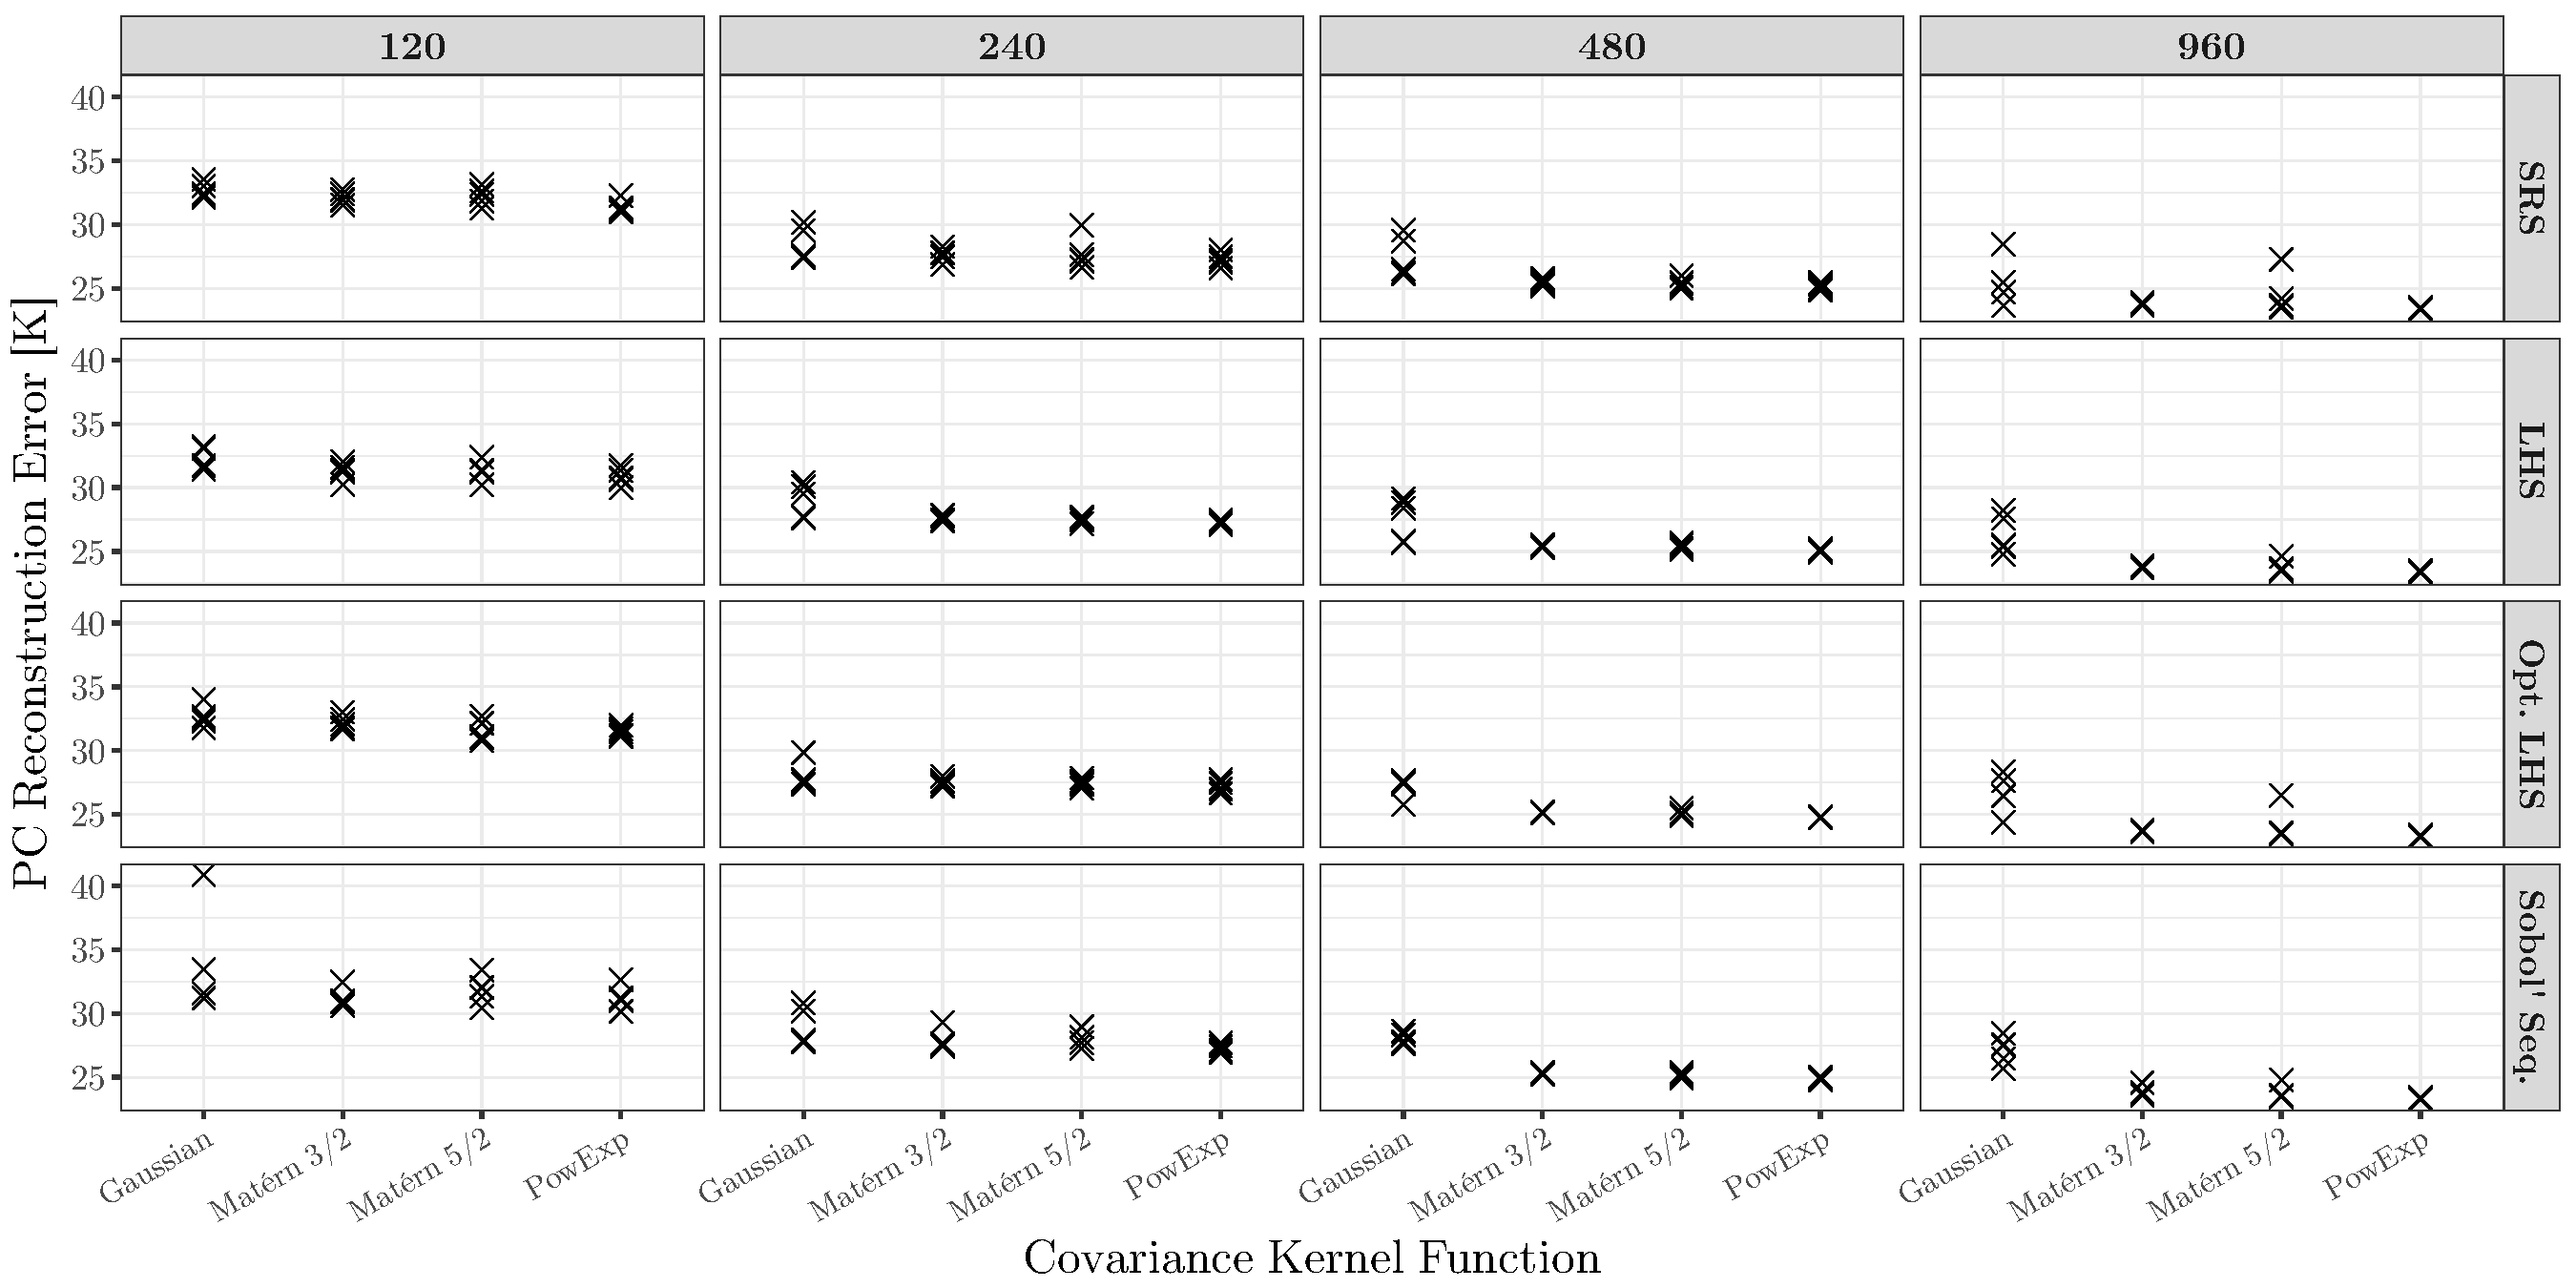
\includegraphics[width=1.0\textwidth]{../figures/chapter4/figures/plotPCGPConstructionTC}
	\caption[The effect of training sample size, experimental design, and covariance function on the predictive performance of GP PC metamodel with respect to the clad temperature output]{The effect of training sample size, experimental design, and covariance function on the predictive performance (in terms of \gls[hyper=false]{rmse}) of \gls[hyper=false]{gp} \gls[hyper=false]{pc} metamodel with respect to the clad temperature output $TC$. $7$ \glspl[hyper=false]{pc} were used for the reconstruction.}
	\label{fig:ch4_plot_pc_gp_construction_tc}
\end{sidewaysfigure}

% Describing the figure itself (as it is the first time it appears)
Fig.~\ref{fig:ch4_plot_pc_gp_construction_tc} summarizes the effect of different training sample sizes, types of experimental design, and types of covariance kernel function on the performance of the constructed \gls[hyper=false]{gp} \gls[hyper=false]{pc} metamodels to predict the clad temperature output.
The training samples were replicated five times for each size and for each design.
The predictive performance was assessed in terms of the \gls[hyper=false]{rmse} which was computed by retaining the first seven \glspl[hyper=false]{pc} and using the validation data set.
Therefore, the \gls[hyper=false]{rmse} shown in the figure represents the combined error due to \gls[hyper=false]{pc} truncation and misprediction of the \gls[hyper=false]{pc} scores.

% Describing the finding in the figure
The size of the training sample was the most important factor in determining the predictive performance of a \gls[hyper=false]{gp} \gls[hyper=false]{pc} metamodel.
The choice of covariance function had some effects on the perfomance especially between the smoother covariance functions (i.e., the Gaussian and the Mate\'rn $5/2$) and the less smooth ones (i.e, the power exponential and the Mate\'rn $3/2$).
\gls[hyper=false]{gp} metamodel constructed using the Gaussian covariance kernel function, in particular,
exhibited significant variation in the performance of training sample replications compared to the other covariance kernel functions.
Finally, the choice of experimental design for the training sample had a negligible effect on the predictive performance of the \gls[hyper=false]{gp} metamodel.

% The Pressure Drop Output
The \gls[hyper=false]{gp} \gls[hyper=false]{pc} metamodel to predict the pressure drop output showed the same behavior of being more difficult to fit for the higher \glspl[hyper=false]{pc} (See Fig.~\ref{fig:ch4_plot_pc_q2_dp}).
\marginpar{\gls[hyper=false]{gp} \gls[hyper=false]{pc} metamodel, pressure drop output}
The \gls[hyper=false]{gp} metamodel for the first standardized \gls[hyper=false]{pc} score remained the easiest to fit.
However, the metamodel of the higher \gls[hyper=false]{pc} better converged than that for the clad temperature output.
That is,
a metamodel with decent predictive performance could be obtained for all first $10$ standardized \glspl[hyper=false]{pc} scores using the considered sample sizes.
Those $10$ \glspl[hyper=false]{pc} carried close to $100\%$ of the total output variance.
\bigfigure[pos=!tbhp,
					 opt={width=0.85\textwidth},
           label={fig:ch4_plot_pc_q2_dp},
           shortcaption={Convergence of \gls[hyper=false]{pc} metamodel with increasing number of training samples with respect to the standardized \glspl[hyper=false]{pc} scores associated with the pressure drop output}]
{../figures/chapter4/figures/plotPCQ2DP}
{Convergence of \gls[hyper=false]{pc} metamodel with increasing number of training samples with respect to the \glspl[hyper=false]{pc} scores associated with the pressure drop output and the $Q_2$ validation metric. The number inside parentheses is the explained variance of the output by the \gls[hyper=false]{pc} and the cumulative explained variance of the first $10$ \glspl[hyper=false]{pc} is about $99\%$.}

% The Liquid carryover output
Finally, the liquid carryover output was found to be the easiest to construct.
\marginpar{\gls[hyper=false]{gp} \gls[hyper=false]{pc} metamodel, liquid carryover output}
While the predictive performance of the \gls[hyper=false]{gp} metamodel with respect to the pressure drop output converged faster across the first five \gls[hyper=false]{pc} scores (Fig.~\ref{fig:ch4_plot_pc_q2_dp}), those \glspl[hyper=false]{pc} of the liquid carryover output contained almost all of the total output variance (Fig.~\ref{fig:ch4_plot_pc_q2_co}).
\bigfigure[pos=!tbhp,
					 opt={width=0.85\textwidth},
           label={fig:ch4_plot_pc_q2_co},
           shortcaption={Convergence of \gls[hyper=false]{gp} metamodel with increasing number of training samples with respect to the standardized \glspl[hyper=false]{pc} scores associated with the liquid carryover output}]
{../figures/chapter4/figures/plotPCQ2CO}
{Convergence of \gls[hyper=false]{gp} metamodel with increasing number of training samples with respect to the standardized \glspl[hyper=false]{pc} scores associated with liquid carryover output and the $Q_2$ validation metric. The number inside parentheses is the explained variance of the output by the \gls[hyper=false]{pc} and the cumulative explained variance of the first five \glspl[hyper=false]{pc} is about $99\%$.}


% Describing finding in the figure, pressure drop output
The effect of different training sample sizes, types of experimental design, and types of covariance kernel function on the predictive performance of the constructed \gls[hyper=false]{gp} \gls[hyper=false]{pc} were also investigated with respect to the pressure drop and the liquid carryover outputs.
Ten and five \glspl[hyper=false]{pc} were used to compute the predicted reconstruction error for the pressure drop and the liquid carryover outputs, respectively. 
The findings for these two outputs were also similar to the ones for the clad temperature output:
the training sample size was the most important factor in determining the predictive performance,
there was a relatively minor effect of the choice of covariance kernel functions especially in terms of the performance variation (with an exception of the Gaussian kernel function which has the worst performance in terms of consistency across replications),
and the choice of experimental design was relatively noninfluential.
Figs.~\ref{fig:ch4_plot_pc_gp_construction_dp} and~\ref{fig:ch4_plot_pc_gp_construction_co} in the appendix summarize these effects for the two outputs.  

%Fig,~\ref{fig:ch4_plot_pc_gp_construction_dp} presents the summary of the effect of different factors in the construction of a \gls[hyper=false]{gp} metamodel with the pressure drop output as its output.
%The reconstruction error was computed using the first $10$ \glspl[hyper=false]{pc}.
%The findings were mostly consistent with the previous results for the clad temperature output.
%The Gaussian covariance kernel function, as before, had the least stable performance across replication especially when combined with latin hypercube type of experimental design.
%Except for that, most of the factors considered converged to the same value of the reconstruction error with less variation across replication compared to the clad temperature output.


% Describing finding in the figure, liquid carryover output
%As before, Fig.~\ref{fig:ch4_plot_pc_gp_construction_co} summarizes the effect of different factor in the construction of a \gls[hyper=false]{gp} metamodel with the liquid carryover output as its output.
%The reconstruction error was computed using the first $5$ \glspl[hyper=false]{pc}.


